\documentclass[11pt]{article}
\usepackage{lmodern}
\usepackage{amssymb,amsmath}
\usepackage{ifxetex,ifluatex}
%\usepackage{fixltx2e} % provides \textsubscript
\usepackage{xr} % referencing external ducument
\ifnum 0\ifxetex 1\fi\ifluatex 1\fi=0 % if pdftex
  \usepackage[T1]{fontenc}
  \usepackage[utf8]{inputenc}
\else % if luatex or xelatex
  \ifxetex
    \usepackage{mathspec}
  \else
    \usepackage{fontspec}
  \fi
  \defaultfontfeatures{Ligatures=TeX,Scale=MatchLowercase}
\fi
% use upquote if available, for straight quotes in verbatim environments
\IfFileExists{upquote.sty}{\usepackage{upquote}}{}
% use microtype if available
\IfFileExists{microtype.sty}{%
\usepackage{microtype}
\UseMicrotypeSet[protrusion]{basicmath} % disable protrusion for tt fontshttps://de.overleaf.com/project/5e85b0680d0bed00011ea790
}{}
\usepackage[margin=1in]{geometry}
\usepackage{hyperref}
\hypersetup{unicode=true,
            pdftitle={Title: Limitations to the Human Neandertal Admixture dating Supplements},
            pdfauthor={Leonardo Nicola Martin Iasi (Max Planck Institute for Evolutionary Anthropology, MPI EVA), Dr.~Benjamin Marco Peter (MPI EVA, benjamin\_peter@eva.mpg.de)},
            pdfborder={0 0 0},
            breaklinks=true}
\urlstyle{same}  % don't use monospace font for urls
 
%\usepackage{natbib}
%\bibliographystyle{References/my_abbrvnat}
%\setcitestyle{authoryear,open={(},close={)}}

\usepackage{graphicx,grffile}
\makeatletter
\def\maxwidth{\ifdim\Gin@nat@width>\linewidth\linewidth\else\Gin@nat@width\fi}
\def\maxheight{\ifdim\Gin@nat@height>\textheight\textheight\else\Gin@nat@height\fi}
\makeatother
% Scale images if necessary, so that they will not overflow the page
% margins by default, and it is still possible to overwrite the defaults
% using explicit options in \includegraphics[width, height, ...]{}

\setkeys{Gin}{width=\maxwidth,height=\maxheight,keepaspectratio}
\IfFileExists{parskip.sty}{%
\usepackage{parskip}
}{% else
\setlength{\parindent}{0pt}
\setlength{\parskip}{6pt plus 2pt minus 1pt}
}
\setlength{\emergencystretch}{3em}  % prevent overfull lines
\providecommand{\tightlist}{%
  \setlength{\itemsep}{0pt}\setlength{\parskip}{0pt}}
\setcounter{secnumdepth}{0}
% Redefines (sub)paragraphs to behave more like sections
\ifx\paragraph\undefined\else
\let\oldparagraph\paragraph
\renewcommand{\paragraph}[1]{\oldparagraph{#1}\mbox{}}
\fi
\ifx\subparagraph\undefined\else
\let\oldsubparagraph\subparagraph
\renewcommand{\subparagraph}[1]{\oldsubparagraph{#1}\mbox{}}
\fi



\usepackage{setspace}
\onehalfspacing
\usepackage[left]{lineno}
\linenumbers
\usepackage[none]{hyphenat}
\usepackage{amsfonts}
\usepackage{amssymb}
\usepackage{graphicx}
\usepackage{float}
\usepackage{xcolor}

\floatplacement{figure}{H}
\begin{document}

\begin{titlepage}


    \vspace*{1cm}
        
        
    \begin{center}       
        \large
        \vspace{1cm}
        An extended admixture pulse model reveals the limits to the dating of Human-Neandertal introgression
        
       \vspace{1.0cm}
        \large
        Iasi, Leonardo N. M. \textsuperscript{1,2} and Peter , Benjamin M. \textsuperscript{1,3} \\ 
        
        \vspace{1.0cm}
            \Huge
            \textbf{Supplement Material}
    \end{center} 

            

\end{titlepage}
\section{Extended Pulse Model}

In this section, we describe in detail the derivation of the extended pulse model, where the gene flow over time is modeled as a Gamma distribution with shape parameter $k$ and scale parameter $\frac{k}{t_m}$. Here, $L_i$ is the length of a segment entered at time $T_i$. We assume each segment length at time $T_i$ to be described by an exponential distribution.

To get the likelihood function for the segment length distribution $P(L_i)$ under the extended pulse we have to solve the following integral:

\begin{equation}
\label{eq:Likelihood_function_extended_pulse_1}
    P(L_i=l) = \int_{0}^{\infty} \frac{1}{\Gamma(k)(\frac{t_m}{k})^k}t^{k-1}e^{-t\frac{k}{t_m}}\ t\ e^{-tl} \ dt 
\end{equation}

we can factor out all terms not depending on $t$:

\begin{equation}
\label{eq:Likelihood_function_extended_pulse_2}
    P(L=l) = \frac{1}{\Gamma(k)(\frac{t_m}{k})^k}\ \int_{0}^{\infty}\ t^{k-1}e^{-t\frac{k}{t_m}}\ t\ e^{-tl} \ dt 
\end{equation}

 
we can re-write the integral into the  form of the known integral $\int_{0}^{\infty}\ x^n e^{-\alpha x} \ dx= \frac{\Gamma{n+1}}{\alpha^{n+1}}$

\begin{equation}
\begin{split}
\label{eq:Likelihood_function_extended_pulse_3}
    P(L=l) &= \frac{1}{\Gamma(k)(\frac{t_m}{k})^k}\ \int_{0}^{\infty}\ t^{k}e^{-(l+\frac{k}{t_m})t} \ dt \\ 
    P(L=l) &= \frac{1}{\Gamma(k)(\frac{t_m}{k})^k}\ \frac{\Gamma(k+1)}{(l+\frac{k}{t_m})^{k+1}} 
\end{split}
\end{equation}

since $\frac{\Gamma(k+1)}{\Gamma(k)} =k$ we can re-write the likelihood to:



\begin{equation}
\begin{split}
\label{eq:Likelihood_function_extended_pulse_final}
    P(L=l) &= \frac{k}{(\frac{t_m}{k})^k \ (l+\frac{k}{t_m})^{k+1}} \\
    &= \frac{k(\frac{k}{t_m})^k} {(l+\frac{k}{t_{m}})^{k+1}}  \\
    &= \frac{k^{k+1}} { t_{m}^k \ (l+\frac{k}{t_{m}})^{k+1}}  \\
    &= t_{m} \ \Bigg( \frac{k}{t_{m}(l+\frac{k}{t_{m}})}\Bigg)^{k+1} \\
    P(L=l) &= t_{m}^{-k} \ \Bigg( \frac{k}{(l+\frac{k}{t_{m}})}\Bigg)^{k+1}
\end{split}
\end{equation}


\section{Supplement Figures}

\begin{figure}
\centering
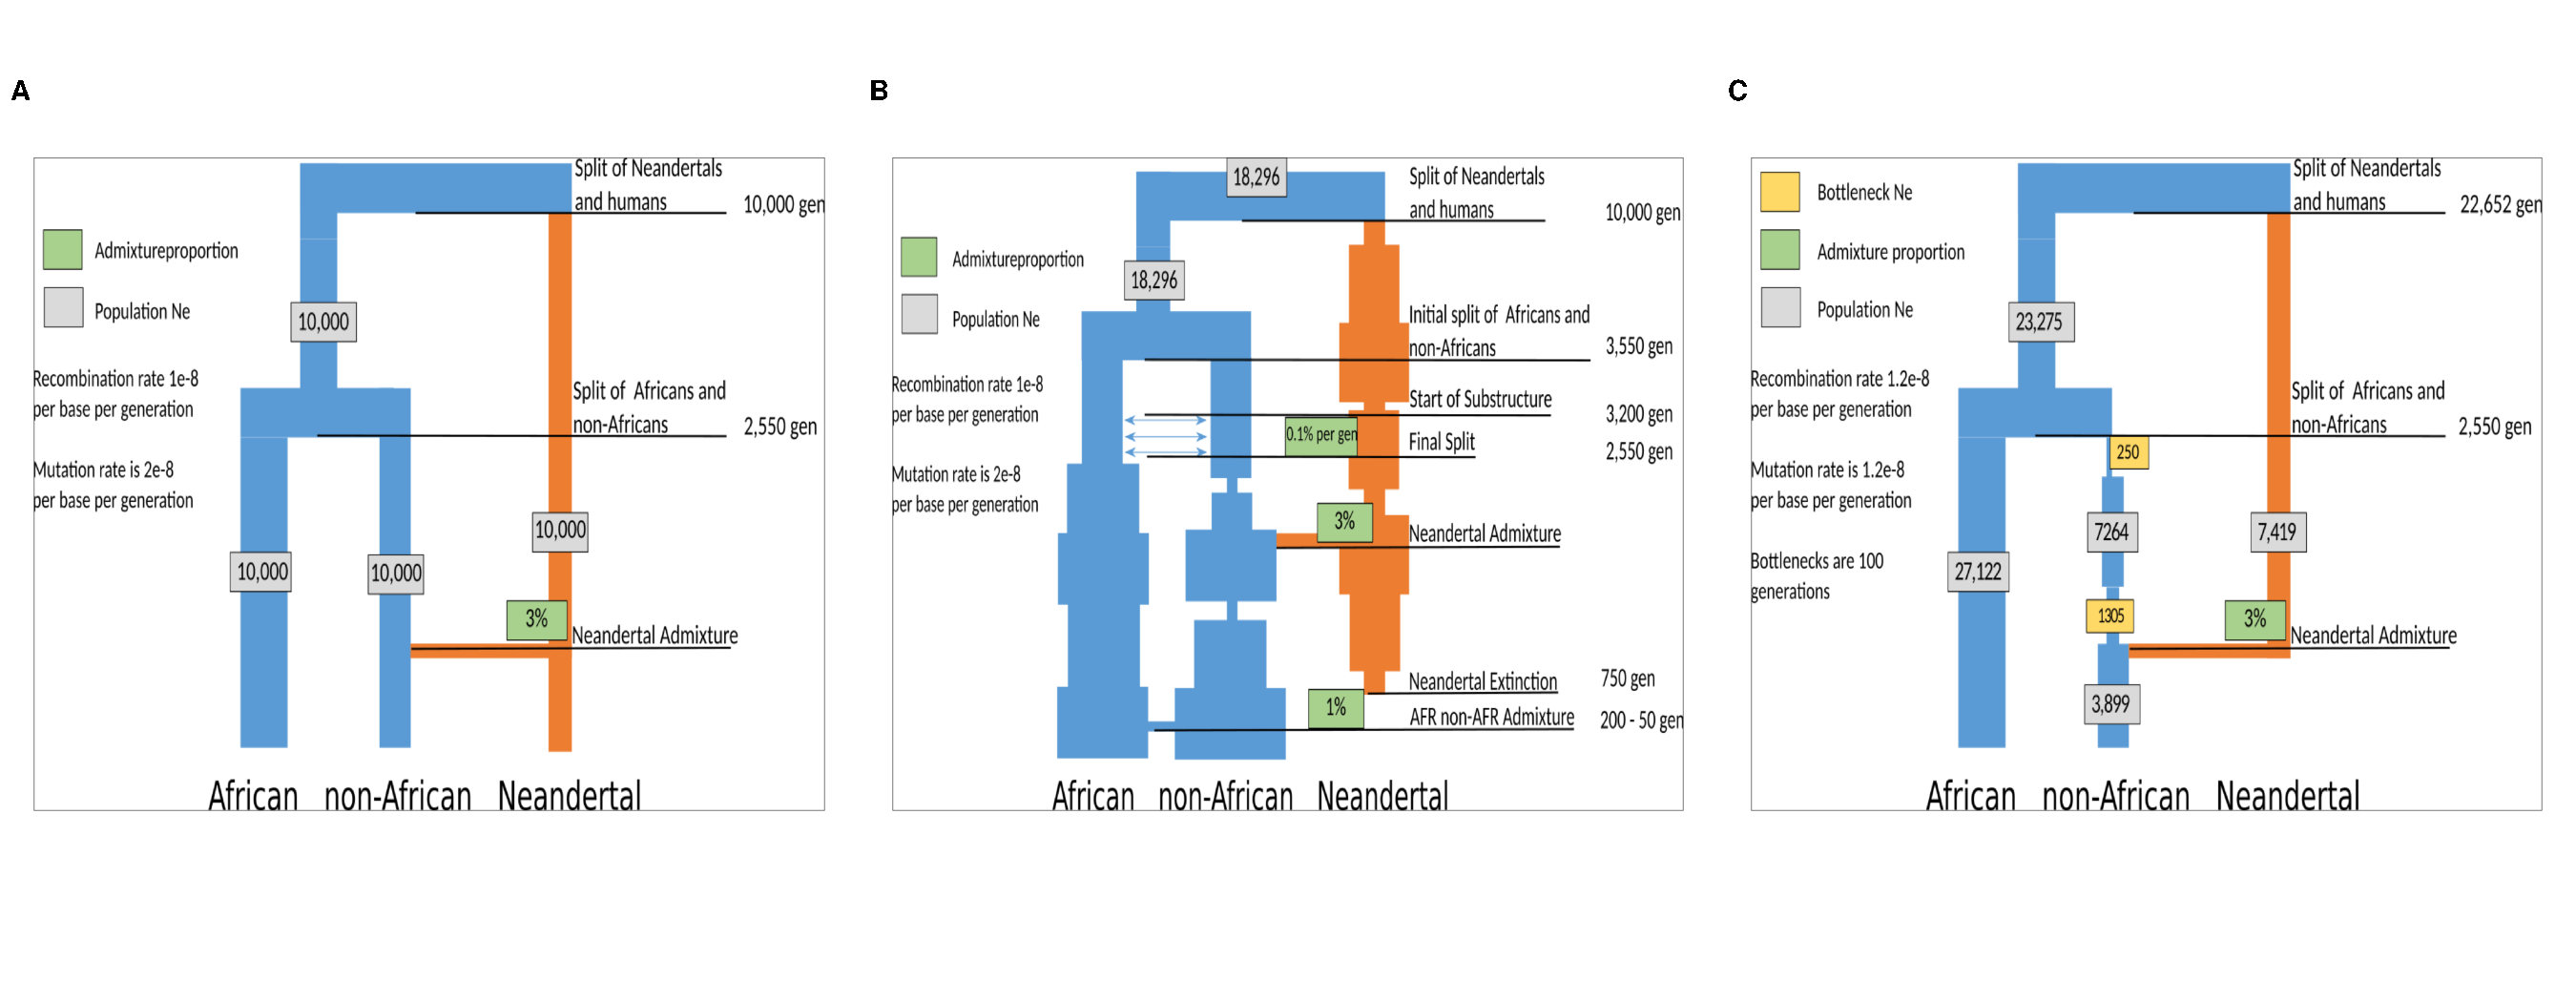
\includegraphics{Admixture_Time_Inference_Paper_Draft_files/figure-latex/All_3_demo_models.pdf}
\caption{\label{fig:figS1} Demographic models of Neandertal introgression into non-Africans used for the simulations. A) Simple demographic model used for ALD simulations with constant population sizes. B) Complex demographic model with substructure in Africa, where after an initial earlier split and isolation the structured population exchange migrants till the final split and additional gene flow between Africans and non-Africans after the Neandertal admixture. The  population sizes after the (final) split are taken from MSMC/PSMC estimates for the respective populations.}
\end{figure}

\begin{figure}
\centering
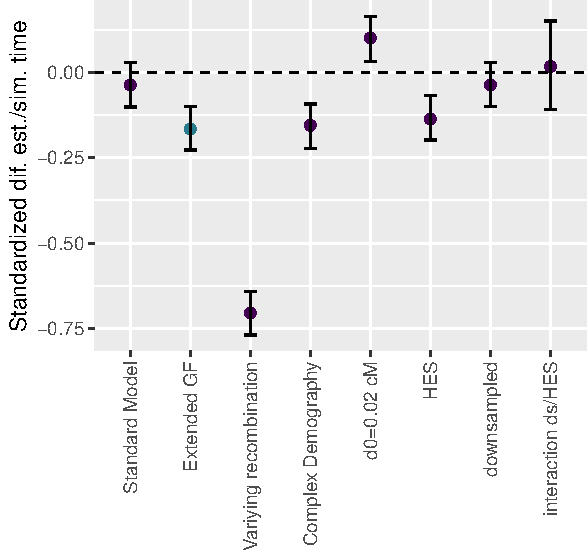
\includegraphics[width=8cm,height=16cm,keepaspectratio]{ATE_Revisions_files/figure-latex/fig3_2-1.pdf}
\caption{\label{fig:figS2_1} GLM effect size estimates and 95\% C.I. for the parameters: gene flow model (simple/extended), recombination rate (constant/varying), demography (simple/complex), minimal genetic distance (0.02/0.05 cM), SNPs used for ALD calculation (100 \% / 5 \%), ascertainment scheme (LES/HES) and additionally the interaction between ascertainment scheme and SNPs used for ALD calculation, on the standardized difference between simulated and estimated admixture time. Estimates are calculated across all possible combinations of parameters and are given as the estimate of the standard model plus the respective parameter estimate. Dotted horizontal line indicates unbiased admixture estimates.}
\end{figure}

\begin{figure}
\centering
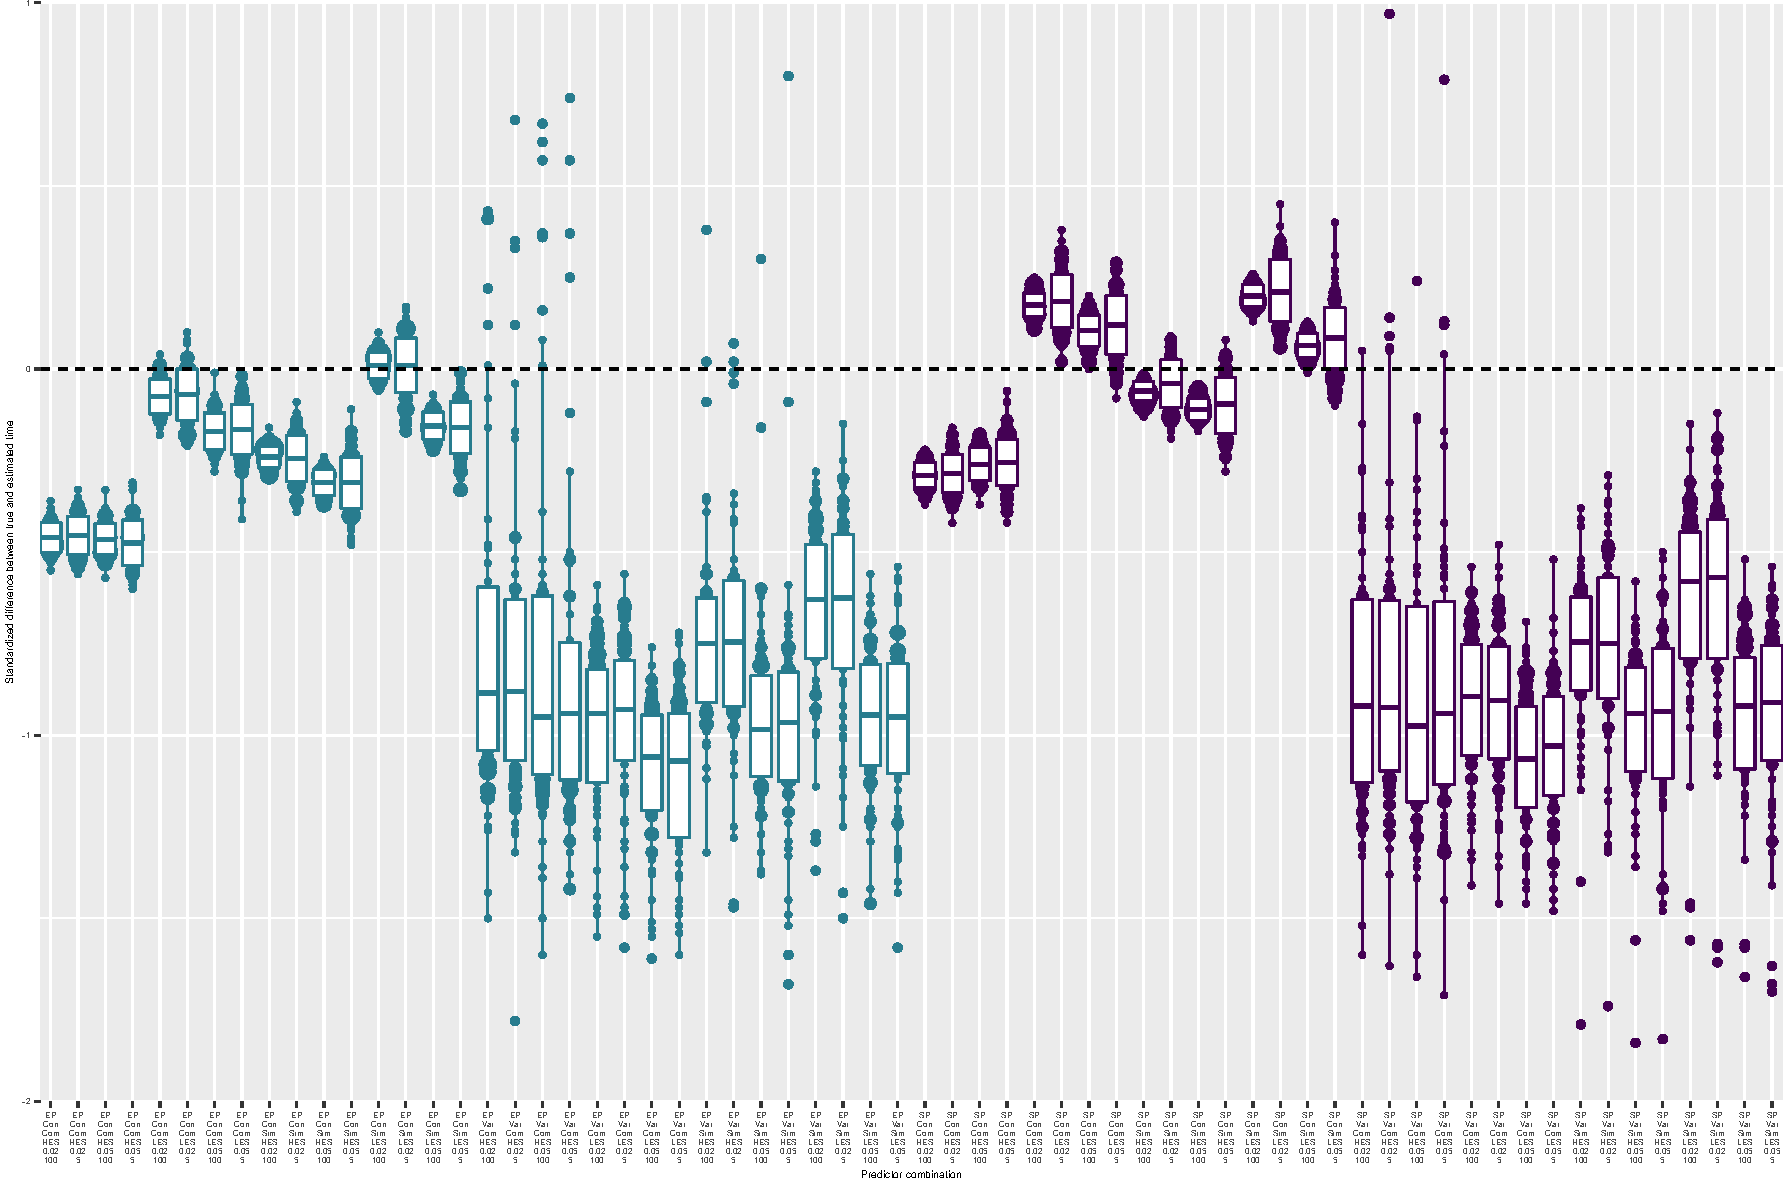
\includegraphics[width=16cm,height=18cm,keepaspectratio]{ATE_Revisions_files/figure-latex/figS2_updated-1.pdf}
\caption{\label{fig:figS2_2} Comparison of the standardized difference between true and estimated admixture time for simulations of all combinations of parameters: ascertainment scheme = LES/HES,  $d_{0}$ = 0.02/0.05 cM, demography = simple/complex, recombination = constant/variable, SNP used 100 \% / 5 \% and the gene flow model = simple/extended. Simulations under the simple pulse are indicated in purple, extended pulse in turquoise. Each simulation was repeated 100 times. Dotted horizontal line indicates no difference between true and estimated time.}
\end{figure}

\begin{figure}
\centering
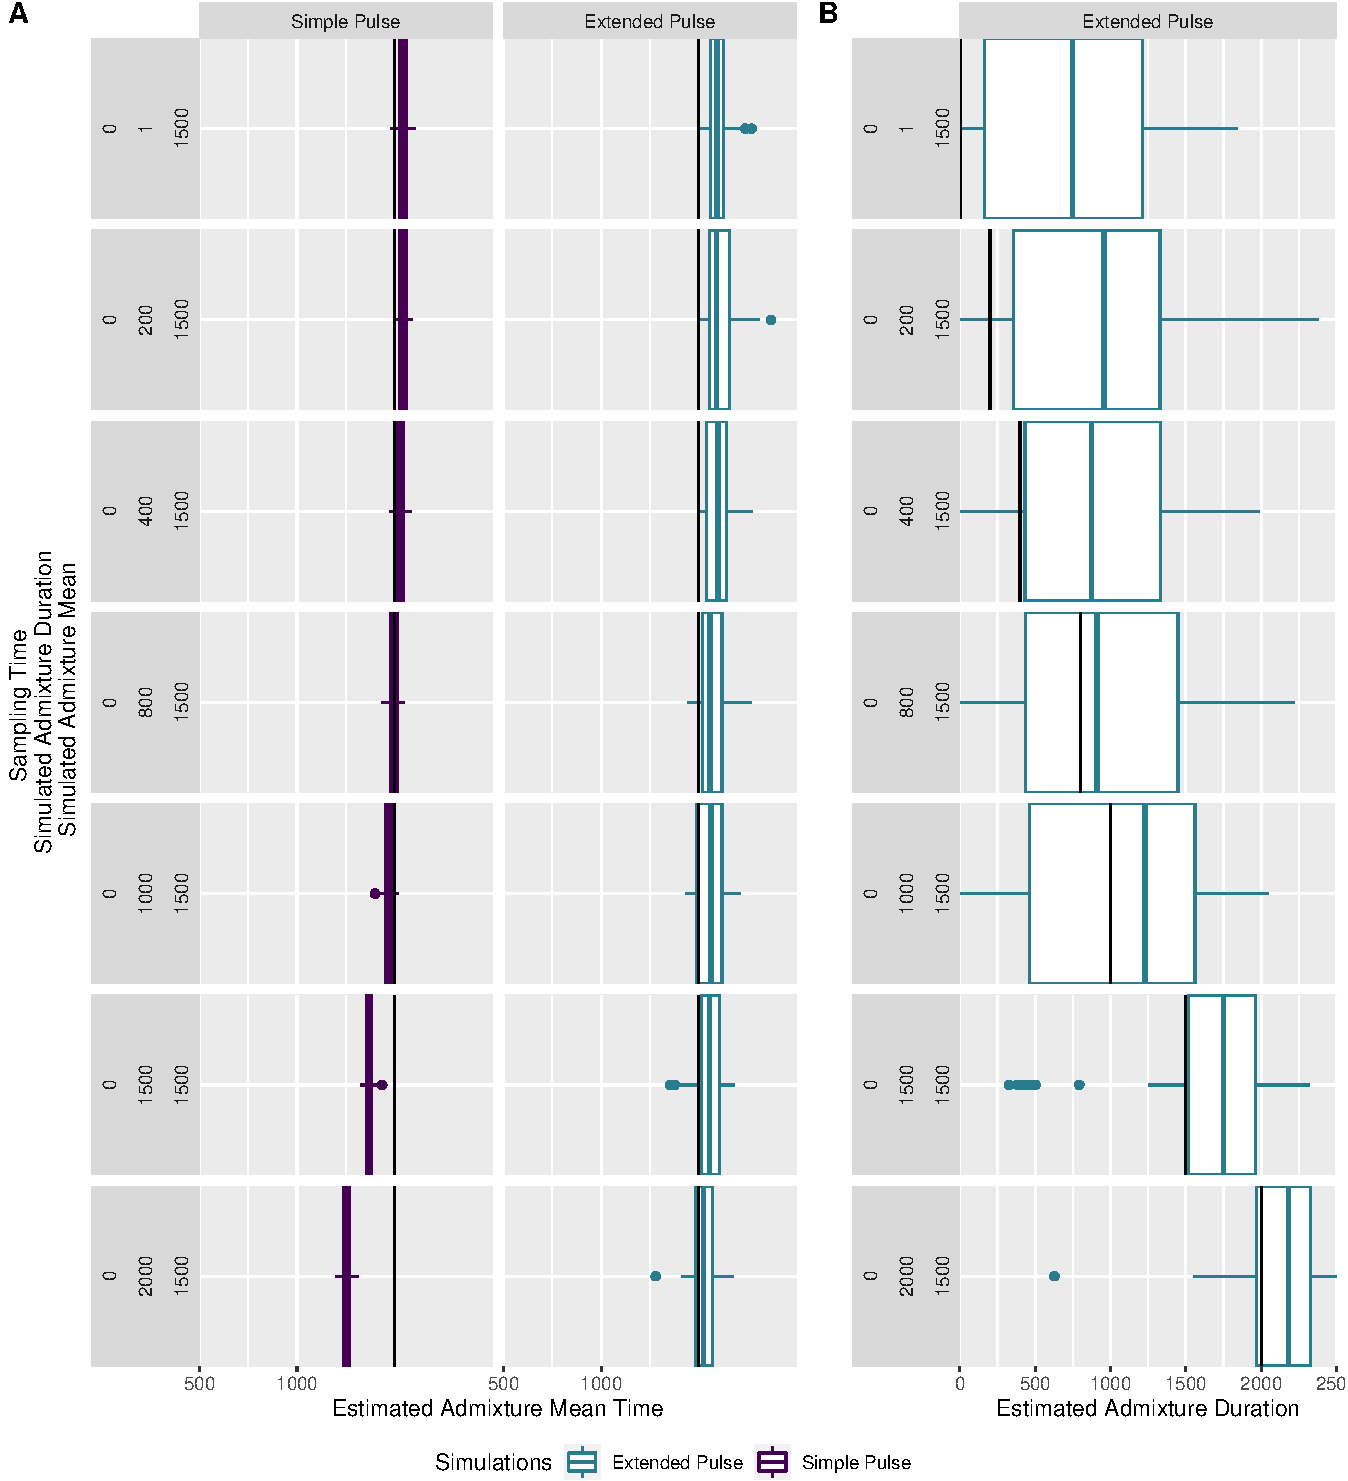
\includegraphics{ATE_Revisions_files/figure-latex/figR3_1-1.pdf}
\caption{\label{fig:figS3} Simple and extended pulse fitted to ALD data for different gene flow durations with mean admixture time at 1500 gnerations ago. A) Mean time estimates. B) Duration estimate.}
\end{figure}

\begin{figure}
\centering
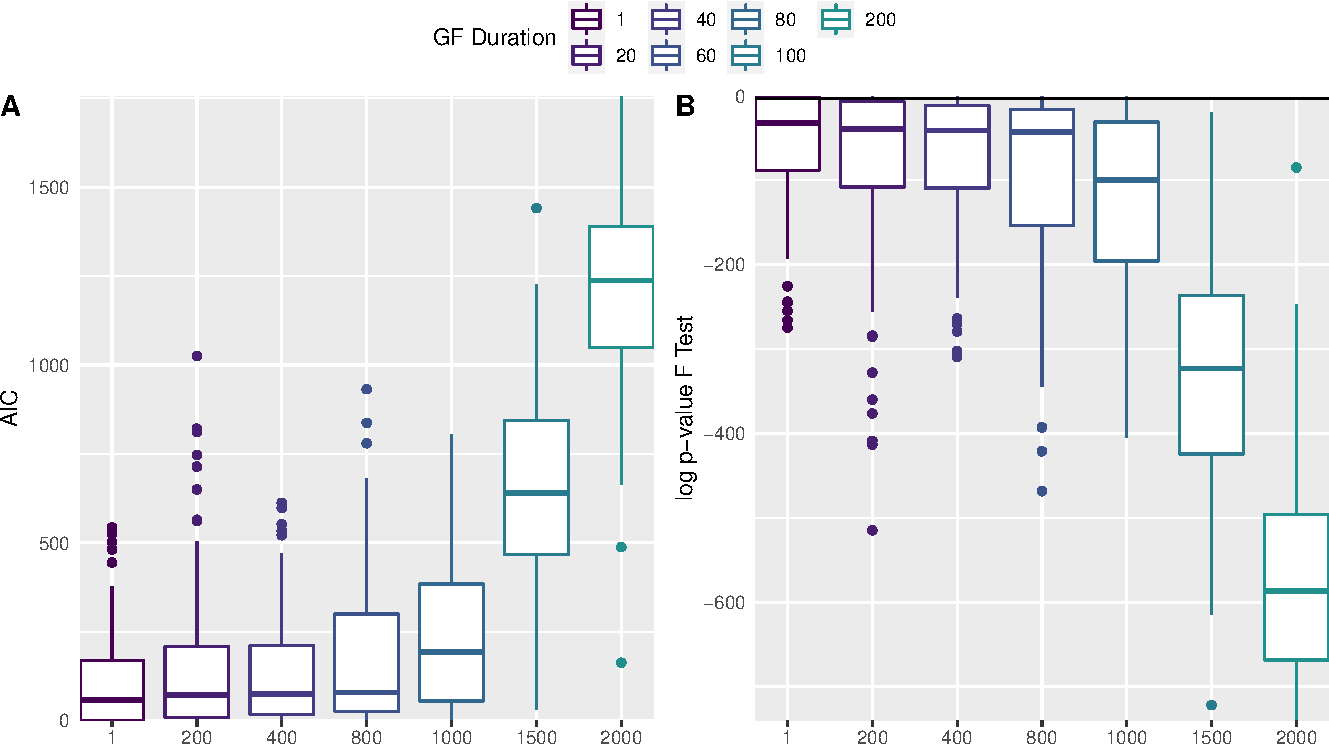
\includegraphics{ATE_Revisions_files/figure-latex/figR3_3-1.pdf}
\caption{\label{fig:figS4} Log likelihood ratio between the simple and extended pulse fitted to ALD data for different gene flow durations with mean admixture time at 1500 gnerations ago.}
\end{figure}

\begin{figure}
\centering
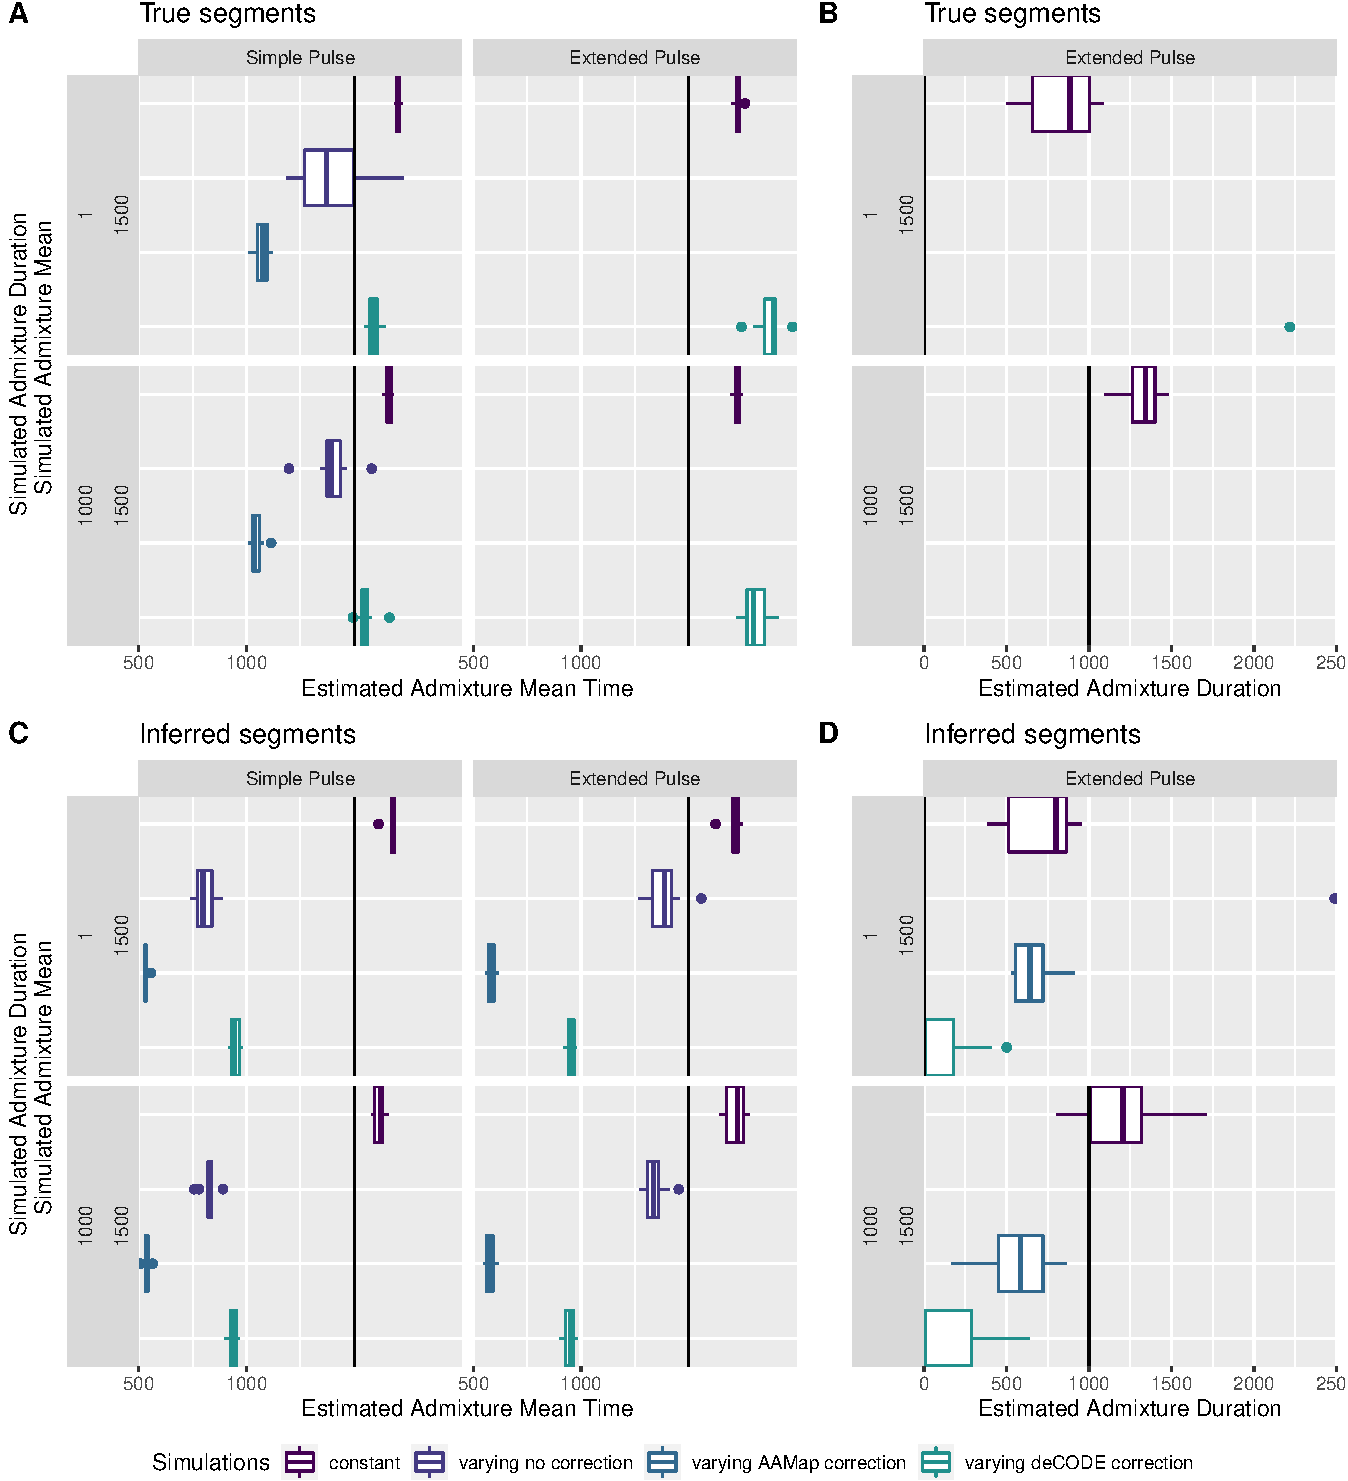
\includegraphics{ATE_Revisions_files/figure-latex/figR3_4-1.pdf}
\caption{\label{fig:figS5} Simple and extended pulse fitted to true and inferred segment data for different gene flow durations with mean admixture time at 1500 generations ago. The simulations used either a constant recombination rate or the deCODE map. The genetic distance is assigned using a constant rate, the AAMap or thye deCODE map. A) Mean time estimates. B) Duration estimate.}
\end{figure}

\begin{figure}
\centering
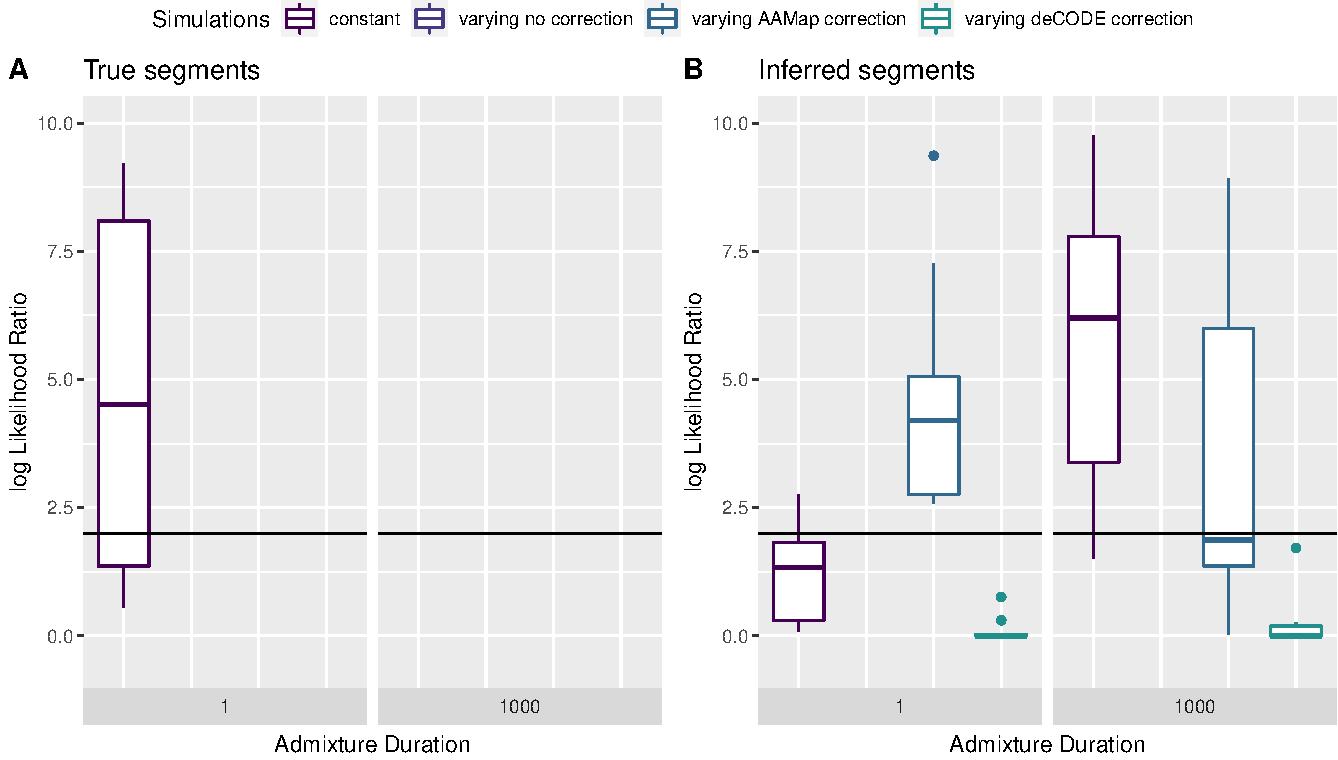
\includegraphics{ATE_Revisions_files/figure-latex/figR3_5-1.pdf}
\caption{\label{fig:figS6} Log likelihood ratio between the simple and extended pulse fitted to true and inferred segment data for different gene flow durations with mean admixture time at 1500 gnerations ago.}
\end{figure}

\section{Supplement Tables}

\begin{table}[H]

\caption{\label{tab:tableS1} Mean, standard deviation, 5.5/94.5 compatibility interval of the posterior distribution for every parameter effect on the standardized difference between true and estimated admixture time.}
\centering
\begin{tabular}{l|r|r|r|r|r|r}
\hline
  & mean & sd & 5.5\% & 94.5\% & n\_eff & Rhat\\
\hline
a & 0.12 & 0.02 & 0.08 & 0.16 & 1220.94 & 1\\
\cline{1-7}
bG & -0.31 & 0.02 & -0.34 & -0.28 & 1559.84 & 1\\
\cline{1-7}
bR & -1.73 & 0.02 & -1.76 & -1.70 & 2112.69 & 1\\
\cline{1-7}
bD & -0.22 & 0.02 & -0.25 & -0.19 & 2036.66 & 1\\
\cline{1-7}
bm & 0.13 & 0.02 & 0.10 & 0.17 & 1657.66 & 1\\
\cline{1-7}
bA & -0.32 & 0.02 & -0.35 & -0.29 & 1721.62 & 1\\
\cline{1-7}
sigma & 0.46 & 0.01 & 0.44 & 0.47 & 2239.47 & 1\\
\hline
\end{tabular}
\end{table}


\begin{table}[H]

\caption{\label{tab:tableS2} Mean and 2.5/97.5 compatibility interval for every parameter estimated in the model fit}
\centering
\begin{tabular}[t]{l|l|l|l}
\hline
Model & A & $t_m$ & c\\
\hline
Simple Pulse & 0.018 (0.018 - 0.018) & 1541 (1487 - 1598) & 1e-05 (6e-06 - 1.5e-05)\\
\hline
Extended Pulse (td=1) & 0.018 (0.018 - 0.018) & 1541 (1487 - 1598) & 1e-05 (6e-06 - 1.5e-05)\\
\hline
Extended Pulse (td=100) & 0.018 (0.018 - 0.018) & 1541 (1488 - 1599) & 1e-05 (6e-06 - 1.5e-05)\\
\hline
Extended Pulse (td=200) & 0.018 (0.018 - 0.018) & 1543 (1490 - 1601) & 1e-05 (6e-06 - 1.5e-05)\\
\hline
Extended Pulse (td=400) & 0.018 (0.018 - 0.018) & 1552 (1498 - 1610) & 1e-05 (6e-06 - 1.5e-05)\\
\hline
Extended Pulse (td=800) & 0.018 (0.018 - 0.018) & 1586 (1531 - 1646) & 1e-05 (5e-06 1.4e-05)\\
\hline
Extended Pulse (td=1000) & 0.018 (0.018 - 0.018) & 1613 (1557 - 1673) & 9e-06 (5e-06 - 1.3e-05)\\
\hline
Extended Pulse (td=1500) &  0.018 (0.018 - 0.018) & 1713 (1654 - 1777) & 7e-06 (3e-06 - 1.1e-05)\\
\hline
Extended Pulse (td=2000) & 0.018 (0.018 - 0.018) & 1875 (1809 - 1945) & 4e-06 (0 - 8e-06)\\
\hline
Extended Pulse (td=2500) & 0.018 (0.018 - 0.018) & 2129 (2055 - 2208) & -1e-06 (-5e-06 - 4e-06)\\
\hline
\end{tabular}
\end{table}

\end{document}